\ssection[Executive Summary]{Executive Summary}

\begin{multicols}{2}

During the last 60 years, Europe has become a distinct political and economic structure. Culturally and linguistically it is rich and diverse. However, from Portuguese to Polish and Italian to Icelandic, everyday communication between Europe’s citizens, within business and among politicians is inevitably confronted with language barriers. The EU's institutions spend about a billion euros a year on maintaining their policy of multilingualism, i.\,e., translating texts and interpreting spoken communication. Does this have to be such a burden? Language technology and linguistic research can make a significant contribution to removing the linguistic borders. Combined with intelligent devices and applications, language technology will help Europeans talk and do business together even if they do not speak a common language. 

\boxtext{Language technology builds bridges.}

%start Norwegian
Norway has an export-based economy and is also heavily involved in international humanitarian, diplomatic, cultural, educational, scientific and military activities. 
Therefore, high levels of proficiency in English and other foreign languages are essential tools for Norwegians.
%end Norwegian
But language barriers can bring business to a halt, especially for SMEs who do not have the financial means to reverse the situation. The only (unthinkable) alternative to this kind of a multilingual Europe would be to allow a single language to take a dominant position, to replace all other languages. 
One way to overcome the language barrier is to learn foreign languages. Yet without technological support, mastering the 23 official languages of the member states of the European Union and some 60 other European languages is an insurmountable obstacle for Europe’s citizens, economy, political debate, and scientific progress. 

The solution is to build key enabling technologies: language technologies will offer European stakeholders tremendous advantages, not only within the common European market, but also in trade relations with non-European countries, especially emerging economies. Language technology solutions will eventually serve as a unique bridge between Europe's languages. An indespensable prerequisite for their development is first to carry out a systematic analysis of the linguistic particularities of all European languages, and the current state of language technology support for them.  
    
The automated translation and speech processing tools currently available on the market fall short of the envisaged goals. The dominant actors in the field are primarily privately-owned for-profit enterprises based in Northern America. As early as the late 1970s, the EU realised the profound relevance of language technology as a driver of European unity, and began funding its first research projects, such as EUROTRA. At the same time, national projects were set up that generated valuable results, but never led to a concerted European effort. In contrast to these highly selective funding efforts, other multilingual societies such as India (22 official languages) and South Africa (11 official languages) have set up long-term national programmes for language research and technology development. 

The predominant actors in LT today rely on imprecise statistical approaches that do not make use of deeper linguistic methods and knowledge. For example, sentences are often automatically translated by comparing each new sentence against thousands of sentences previously translated by humans. The quality of the output largely depends on the size and quality of the available  data. While the automatic translation of simple sentences in languages with sufficient amounts of available textual data can achieve useful results, shallow statistical methods are doomed to fail in the case of languages with a much smaller body of sample data or in the case of sentences with complex, non-repetitive structures. Analysing the deeper structural properties of languages is the only way forward if we want to build applications that perform well across the entire range of European languages.

\boxtext{Language technology as a key for the future}

The European Union is thus funding projects such as EuroMatrix and EuroMatrixPlus (since 2006) and iTranslate4 (since 2010) that carry out basic and applied research, and generate resources for establishing high quality language technology solutions for all European languages. 
European research in the area of language technology has already achieved a number of successes. For example, the translation services of the European Union now use the Moses open-source machine translation software, which has been mainly developed in European research projects. The Verbmobil project, funded by the German Ministry of Education and Research (BMBF) between 1993 and 2000, pushed Germany into the lead in the world of speech translation research for a time. Many of the research and development labs located in Germany at the time (e.\,g., IBM and Philips) have since been closed down or moved elsewhere. Rather than building on the outcomes of these research projects, Europe has tended to pursue isolated research activities with a less pervasive impact on the market. The economic value of even the earliest efforts can be seen in the number of spin-offs. A company such as Trados, which was founded back in 1984, was sold to the UK-based SDL in 2005.

\boxtext{Language Technology helps unify Europe}

Drawing on the insights gained so far, today’s hybrid language technology mixing deep processing with statistical methods should be able to bridge the gap between all European languages and beyond. But as this series of white papers shows, there is a dramatic difference in the state of readiness with respect to language solutions and the state of research between Europe’s member states. 

%start Norwegian
This whitepaper for the Norwegian language demonstrates that on the one hand, Norwegian enjoys a relatively secure position as the national and majority language of a modern European nation. 
Information and Communication Technologies (ICT) have permeated all aspects of Norwegian society, and 93\% of the Norwegian population has access to the Internet. 
On the other hand, this general ICT maturity is not accompanied by an equally impressive state of Research and Development (R\&D) within Language Resources and Technologies (LRT). 
Language technology presupposes certain basic resources (word lists, text corpora, speech corpora) to enable the development of language technology products. 
Basic resources, as well as the resulting products, are just as costly and time-consuming to develop for smaller languages as for larger languages; since Norwegian has two official written norms and a wide variety of dialects, the development costs are even higher. 
Thus, Norwegian is not attractive from a commercial point of view and is largely dependent on public funding.

Through a joint effort by the Norwegian Language Council, the Research Council, commercial companies and Norwegian research institutions, there is an emerging political awareness that language technology is important for Norway, not only to be industrially competitive, but also culturally. 
This growing awareness has produced two major milestones in the development of Norwegian LRT.
The first milestone was KUNSTI, the first coordinated Norwegian research program specifically targeting Norwegian LRT (2001–2006). 
It generated twenty research projects, fostered new researchers and produced some basic language resources and tools for Norwegian, although very few of these were made available for general reuse in further R\&D. 
The second milestone was the creation of the \emph{Language Technology Resource Collection for Norwegian -- Språkbanken}, established in 2010 after having been on the agenda for two decades. 
Språkbanken is to function as an infrastructure for making Norwegian LRT available for research and commercial use, thus hopefully reducing the threshold for developing Norwegian LRT products.

The present report reveals that Norwegian is still not by any means as richly endowed with high-quality software applications as English. 
While basic LRTs exist for Norwegian, in some cases they are fragmented and in many cases there are restrictions on their use, incompatibilities and insufficient documentation. Furthermore, many research results are not properly disseminated and many potential users are unaware of their existence. There are also conspicuous gaps, such as the present lack of a national terminology infrastructure, parallel corpora of a sufficient size, and corpora of spontaneous speech with good dialect coverage. 

In the Language Service sector there seems to be an underuse of LRT for Norwegian. 
Potential users of LRT are often aware of the possible benefits of LRT but they do not have the expertise to deploy such systems themselves, and they find it difficult to evaluate the suitability of available LRT. 
Thus, we still have a long way to go in order to ensure the full inclusion of the Norwegian language in our digital information society.
%end Norwegian

META-NET’s vision is high-quality language technology for all languages that supports political and economic unity through cultural diversity. This technology will help tear down existing barriers and build bridges between Europe’s languages. This requires all stakeholders -- in politics, research, business, and society -- to unite their efforts for the future.

This whitepaper series complements the other strategic actions taken by META-NET (see the appendix for an overview). Up-to-date information such as the current version of the META-NET vision paper \cite{Meta1} or the Strategic Research Agenda (SRA) can be found on the META-NET web site: \url{http://www.meta-net.eu}.
\end{multicols}

\clearpage

\ssection[Languages at Risk: a Challenge for Language Technology]{Languages at Risk: a Challenge for Language Technology}

\begin{multicols}{2}

We are witnesses to a digital revolution that is dramatically impacting communication and society. Recent developments in information and communication technology are sometimes compared to Gutenberg’s invention of the printing press. What can this analogy tell us about the future of the European information society and our languages in particular?

\boxtext{We are witnessing a digital revolution that is comparable to Gutenberg’s invention of the printing press.}

After Gutenberg’s invention, real breakthroughs in communication were accomplished by efforts such as Luther’s translation of the Bible into vernacular language. In subsequent centuries, cultural techniques have been developed to better handle language processing and knowledge exchange:

\begin{itemize}
\item the orthographic and grammatical standardisation of major languages enabled the rapid dissemination of new scientific and intellectual ideas;
\item the development of official languages made it possible for citizens to communicate within certain (often political) boundaries;
\item the teaching and translation of languages enabled exchanges across languages;
\item the creation of editorial and bibliographic guidelines assured the quality of printed material;
\item the creation of different media like newspapers, radio, television, books, and other formats satisfied different communication needs. 
\end{itemize}

In the past twenty years, information technology has helped to automate and facilitate many processes:

\begin{itemize}
\item desktop publishing software has replaced typewriting and typesetting;
\item Microsoft PowerPoint has replaced overhead projector transparencies;
\item e-mail allows documents to be sent and received more quickly than using a fax machine;
\item Skype offers cheap Internet phone calls and hosts virtual meetings;
\item audio and video encoding formats make it easy to exchange multimedia content;
\item web search engines provide keyword-based access;
\item online services like Google Translate produce quick, approximate translations;
\item social media platforms such as Facebook, Twitter and Google+ facilitate communication, collaboration, and information sharing.
\end{itemize}

Although these tools and applications are helpful, they are not yet capable of supporting a fully-sustainable, multilingual European society in which information and goods can flow freely.

\subsection[Language Borders Hold back the European Information Society]{Language Borders\newline Hold back the European Information Society}

We cannot predict exactly what the future information society will look like. However, there is a strong likelihood that the revolution in communication technology is bringing together people who speak different languages in new ways. This is putting pressure both on individuals to learn new languages and especially on developers to create new technology applications to ensure mutual understanding and access to shareable knowledge. In the global economic and information space, there is increasing interaction between different languages, speakers and content thanks to new types of media. The current popularity of social media (Wikipedia, Facebook, Twitter, YouTube, and, recently, Google+) shows only the tip of the iceberg.

\boxtext{A global economy and information space confronts us with different languages, speakers and content.}

Today, we can transmit gigabytes of text around the world in a few seconds before we recognise that it is in a language that we do not understand. According to a recent report from the European Commission, 57\% of Internet users in Europe purchase goods and services in languages that are not their native language; English is the most common foreign language followed by French, German and Spanish. 55\% of users read content in a foreign language while 35\% use another language to write e-mails or post comments on the Web \cite{EC1}. A few years ago, English might have been the lingua franca of the Web—the vast majority of content on the Web was in English—but the situation has now drastically changed. The amount of online content in other European (as well as Asian and Middle Eastern) languages has exploded.

Surprisingly, this ubiquitous digital linguistic divide has not gained much public attention; yet, it raises a very pressing question: Which European languages will thrive in the networked information and knowledge society, and which are doomed to disappear?

\subsection{Our Languages at Risk}

While the printing press helped step up the exchange of information in Europe, it also led to the extinction of many European languages. Regional and minority languages were rarely printed and languages such as Cornish and Dalmatian were limited to oral forms of transmission, which in turn restricted their scope of use. Will the Internet have the same impact on our modern languages?

\boxtext{The wide variety of languages in Europe is one of its richest and most important cultural assets.}

Europe’s approximately 80 languages are one of our richest and most important cultural assets, and a vital part of this unique social model \cite{EC2}. While languages such as English and Spanish are likely to survive in the emerging digital marketplace, many European languages could become irrelevant in a networked society. This would weaken Europe’s global standing, and run counter to the strategic goal of ensuring equal participation for every European citizen regardless of language. According to a UNESCO report on multilingualism, languages are an essential medium for the enjoyment of fundamental rights, such as political expression, education and participation in society \cite{Unesco1}.

\subsection{Language Technology is a Key Enabling Technology}

In the past, investments in language preservation focussed primarily on language education and translation. According to one estimate, the European market for translation, interpretation, software localisation and website globalisation was €8.4 billion in 2008 and is expected to grow by 10\% per annum \cite{EC3}. Yet this figure covers just a small proportion of current and future needs in communicating between languages. The most compelling solution for ensuring the breadth and depth of language usage in Europe tomorrow is to use appropriate technology, just as we use technology to solve our transport and energy needs among others.

Language technology targeting all forms of written text and spoken discourse can help people to collaborate, conduct business, share knowledge and participate in social and political debate regardless of language barriers and computer skills. It often operates invisibly inside complex software systems to help us already today to:

\begin{itemize}
\item find information with a search engine;
\item check spelling and grammar in a word processor;
\item view product recommendations in an online shop;
\item follow the spoken directions of a navigation system;
\item translate web pages via an online service.
\end{itemize}

Language technology consists of a number of core applications that enable processes within a larger application framework. The purpose of the META-NET language white papers is to focus on how ready these core enabling technologies are for each European language. 

\boxtext{Europe needs robust and affordable language technology for all European languages.}

To maintain our position in the frontline of global innovation, Europe will need language technology, tailored to all European languages, that is robust and affordable and can be tightly integrated within key software environments. Without language technology, we will not be able to achieve a really effective interactive, multimedia and multilingual user experience in the near future.

\subsection{Opportunities for Language Technology}

In the world of print, the technology breakthrough was the rapid duplication of an image of a text using a suitably powered printing press. Human beings had to do the hard work of looking up, assessing, translating, and summarising knowledge. We had to wait until Edison to record spoken language – and again his technology simply made analogue copies.

Language technology can now simplify and automate the processes of translation, content production, and knowledge management for all European languages. It can also empower intuitive speech-based interfaces for household electronics, machinery, vehicles, computers and robots. Real-world commercial and industrial applications are still in the early stages of development, yet R\&D achievements are creating a genuine window of opportunity. For example, machine translation is already reasonably accurate in specific domains, and experimental applications provide multilingual information and knowledge management, as well as content production, in many European languages. 

As with most technologies, the first language applications such as voice-based user interfaces and dialogue systems were developed for specialised domains, and often exhibit limited performance. However, there are huge market opportunities in the education and entertainment industries for integrating language technologies into games, edutainment packages, libraries, simulation environments and training programmes. Mobile information services, computer-assisted language learning software, eLearning environments, self-assessment tools and plagiarism detection software are just some of the application areas in which language technology can play an important role. The popularity of social media applications like Twitter and Facebook suggest a need for sophisticated language technologies that can monitor posts, summarise discussions, suggest opinion trends, detect emotional responses, identify copyright infringements or track misuse.

\boxtext{Language technology helps overcome the `disability' of linguistic diversity.}

Language technology represents a tremendous opportunity for the European Union. It can help to address the complex issue of multilingualism in Europe – the fact that different languages coexist naturally in European businesses, organisations and schools. However, citizens need to communicate across the language borders of the European Common Market, and language technology can help overcome this final barrier, while supporting the free and open use of individual languages. Looking even further ahead, innovative European multilingual language technology will provide a benchmark for our global partners when they begin to support their own multilingual communities. Language technology can be seen as a form of `assistive' technology that helps overcome the `disability' of linguistic diversity and makes language communities more accessible to each other. Finally, one active field of research is the use of language technology for rescue operations in disaster areas, where performance can be a matter of life and death: Future intelligent robots with cross-lingual language capabilities have the potential to save lives.

\subsection{Challenges Facing Language Technology}

Although language technology has made considerable progress in the last few years, the current pace of technological progress and product innovation is too slow. Widely-used technologies such as the spelling and grammar correctors in word processors are typically monolingual, and are only available for a handful of languages. Online machine translation services, although useful for quickly generating a reasonable approximation of a document’s contents, are fraught with difficulties when highly accurate and complete translations are required. Due to the complexity of human language, modelling our tongues in software and testing them in the real world is a long, costly business that requires sustained funding commitments. Europe must therefore maintain its pioneering role in facing the technological challenges of a multiple-language community by inventing new methods to accelerate development right across the map. These could include both computational advances and techniques such as crowdsourcing.

\boxtext{The current pace of technological progress is too slow.}

\subsection{Language Acquisition in Humans and Machines}

To illustrate how computers handle language and why it is difficult to program them to process different tongues, let’s look briefly at the way humans acquire first and second languages, and then see how language technology systems work.

Humans acquire language skills in two different ways. Babies acquire a language by listening to the real interactions between their parents, siblings and other family members. From the age of about two, children produce their first words and short phrases. This is only possible because humans have a genetic disposition to imitate and then rationalise what they hear. 

Learning a second language at an older age requires more cognitive effort, largely because the child is not immersed in a language community of native speakers. At school, foreign languages are usually acquired by learning grammatical structure, vocabulary and spelling using drills that describe linguistic knowledge in terms of abstract rules, tables and examples.

\boxtext{Humans acquire language skills in two different ways: learning examples and learning the underlying language rules.}

Moving now to language technology, the two main types of systems ‘acquire’ language capabilities in a similar manner. Statistical (or ‘data-driven’) approaches obtain linguistic knowledge from vast collections of concrete example texts. While it is sufficient to use text in a single language for training, e.\,g., a spell checker, parallel texts in two (or more) languages have to be available for training a machine translation system. The machine learning algorithm then learns patterns of how words, short phrases and complete sentences are translated. 

This statistical approach usually requires millions of sentences to boost performance quality. This is one reason why search engine providers are eager to collect as much written material as possible. Spelling correction in word processors, and services such as Google Search and Google Translate, all rely on statistical approaches. The great advantage of statistics is that the machine learns quickly in a continuous series of training cycles, even though quality can vary randomly.

The second approach to language technology, and to machine translation in particular, is to build rule-based systems. Experts in the fields of linguistics, computational linguistics and computer science first have to encode grammatical analyses (translation rules) and compile vocabulary lists (lexicons). This is very time consuming and labour intensive. Some of the leading rule-based machine translation systems have been under constant development for more than 20 years. The great advantage of rule-based systems is that the experts have more detailed control over the language processing. This makes it possible to systematically correct mistakes in the software and give detailed feedback to the user, especially when rule-based systems are used for language learning. However, due to the high cost of this work, rule-based language technology has so far only been developed for a few major languages. 

\boxtext{The two main types of language technology systems acquire language in a similar manner.}

As the strengths and weaknesses of statistical and rule-based systems tend to be complementary, current research focusses on hybrid approaches that combine the two methodologies. However, these approaches have so far been less successful in industrial applications than in the research lab. 

As we have seen in this chapter, many applications widely used in today’s information society rely heavily on language technology, particularly in Europe’s economic and information space. Although this technology has made considerable progress in the last few years, there is still huge potential to improve the quality of language technology systems. In the next section, we describe the role of 
%start Norwegian
Norwegian in European information society and assess the current state of language technology for the Norwegian language.
%end Norwegian
\end{multicols}

\clearpage

%start Norwegian
\ssection[The Norwegian Language in the European Information Society]{The Norwegian Language in the European Information Society}

\begin{multicols}{2}

\subsection{General Facts}

Norwegian is the common spoken and written language in Norway and is the native language of the vast majority of the Norwegian population (more than 90\%) and has about 4,320,000 speakers at present.
It is the normal language of government and administration, of the school system at all levels, of business and of general day-to-day interactions in Norway.
Minority languages (in the sense of the European Charter on Regional and Minority Languages) in Norway are Saami, Kven, Romanes and Norwegian Romani.
Each of these groups represents some hundreds to thousands of speakers \cite{stm35:2008}. 
Norwegian Sign Language is used by approximately 15,000 speakers \cite{Erl:2007}. 
In addition, there are immigrant languages.
Immigrants and those born in Norway to immigrant parents constitute 600,900 persons or 12.2\% of Norway’s population, the majority of the immigrants currently being from Poland, Sweden, Germany and Iraq according to Statistics Norway.

Norwegian is a North Germanic language and is closely related to Danish and Swedish, and these three languages are mutually understandable. 
Norwegian has a large variety of dialects. 
Even though so-called ‘standard East Norwegian’ functions as a de facto standard for normalized speech, such standardization occurs to a far less extent in Norway than in most of the European countries.
Norwegian has two official written standards, Bokmål and Nynorsk. 
Formally, the two written standards are equal in status; in practice Bokmål is by far the most dominant; it is estimated to be used by approximately 87\% of the population \cite{stm35:2008}.
To ensure the continued use of Nynorsk, \textit{Målloven} (the Language Act) regulates the use of the written standards in the public sector, and all pupils learn Bokmål as well as Nynorsk at school, even if there are political movements to abolish this requirement.

\subsection{Particularities of the Norwegian Language}

Norwegian exhibits a number of specific characteristics that contribute to the richness of the language but can also be a challenge for the computational processing of natural language. 

\subsubsection{Challenges in spoken Norwegian}
Spoken Norwegian comprises a wide variety of dialects, which traditionally have a more prominent role than those in other European countries \cite{stm35:2008}.
Since the use of a spoken standard is generally not enforced, speakers use their dialects (sometimes in moderated form) in most oral communication, also in the media.
Dialectal variation represents a challenge for machines when attempting to convert speech into text or text into speech.

The Norwegian compounding system, shared with other Germanic languages, poses a challenge for speech technology as well as for technologies for the written language (see below). 
It allows speakers to join together words quite freely in order to coin new words. 
For instance, the words \textit{aske} (ash), \textit{krise} (crisis) and \textit{pakke} (package) can be compounded into \textit{askekrisepakke}. 
Some of them are only used occasionally, while some represent terminology in specialised domains, and others become lexicalized and are entered into dictionaries. 

Furthermore, most Norwegian dialects have contrastive use of pitch realized as two distinctive word intonations, often called toneme 1 and 2. 
These tonal accents, combined with the lack of a one-to-one relation between sounds and letters in Norwegian, pose a particular challenge to any speech technology. 
Among other things, Norwegian has a wide range of homographic forms which are realized with different tonemes, e.g. \textit{sulten} (‘the hunger’, toneme 1) versus \textit{sulten} (‘hungry’, toneme 2), and it is crucial that a speech synthesis system is able to attribute the right tone to individual tokens of the lexeme, in this case by syntactic disambiguation. 
Converting from text to speech, syntactic disambiguation is needed to distinguish between homographs that differ both tonemically and segmentally, such as the pair \textit{landet} {[}lanE{]} (`the country', toneme 1) versus \textit{landet} {[}lanEt{]} (`landed', toneme 2). 
In fact, most neuter nouns have such verbal homographic counterparts.

\subsubsection{Challenges in written Norwegian}

As regards the written language, the two official Norwegian written standards differ significantly in spelling and word formation, and in some parts of their vocabulary and grammar. 
In practice the bilingual requirement in administrative and educational institutions is sometimes hard to meet, as people experience the differences as hard to learn. 
The effort to maintain this form of bilingualism is very high and the need for proofreading and for accurate translation between the two norms is therefore apparent.

What is more, even within each written standard considerable variation is allowed in the form and inflection of words. 
The word for `extinguish' can for instance be written as \textit{slukke} or \textit{slokke} in Bokmål (\textit{sløkke} or \textit{sløkkje} in Nynorsk), while the past tenses in Bokmål can be \textit{slukket}, \textit{slukka}, \textit{slokket} or \textit{slokka}. 
Although not all possible combinations of words and endings are always used in practice, the combinatory possibilities are still formidable, sometimes leading to thousands of possible ways to write the same sentence. 
To complicate matters further, the Norwegian writing system has not been stable, because a substantial series of spelling reforms have been adopted throughout the years, which means that older language resources need to be updated for use in present day contexts.

As mentioned in the section on spoken particularities, the Norwegian compounding system is a challenge to any language technology because it requires good compound analyzers.
One of the many challenges in machine translation is the use of Norwegian reflexives, as in the following sentence:

\begin{quote}
	\nynorsk{\emph{Per visste ikkje at Kari hadde freista å reparere bilen \emph{sin}.}}
	\bokmaal{\emph{Per visste ikke at Kari hadde forsøkt å reparere bilen \emph{sin}.}}\\
	Per didn’t know that Kari had tried to fix her/*his car.
\end{quote}

A correct translation requires the need for a Norwegian deep grammatical analysis of this sentence.

\subsection{Recent Developments}

In recent years, the standardization of the written language has received much attention. 
During the past decade the Language Council of Norway has adopted a series of resolutions that streamline the written norms and bring them more in line with the observed use of written language. 
The earlier policy of attempting to merge the two written norms has been abandoned and instead variation has been reduced, even if considerable freedom is still allowed.
Foreign films and TV-programs are usually not dubbed into Norwegian (in contrast to many other countries such as Germany and Spain), which means that generations of Norwegians have been strongly exposed to English, especially during their adolescence. 
This exposure has probably increased through the growing use of the Internet. 
Therefore, many Norwegians have good skills in English. 
The presence of English is reflected in loanwords from English, although an investigation of new words in Norwegian newspapers over the past ten years indicates that only about 5\% of those come from English \cite{And:2011}.

Nevertheless, language policy makers have expressed a serious concern \cite{nih:2005} that Norwegian is losing ground in particular domains, for instance in ICT, business, financial and administrative domains. 
A so-called domain loss means that another language (English, in our case) becomes the primary language within a certain domain, which means that Norwegian terms are no longer produced in this domain. 
As a result, Norwegian may become partly dysfunctional as a means of communication between field experts or between experts and the general public. 
Ironically, the absence of satisfactory Norwegian terms may cause language users to develop a general attitude that it is easier to express something in English. 

Since the use of a non-mother tongue naturally impedes the ability to express oneself correctly and efficiently, it is important to raise awareness of a development that runs the risk of excluding parts of the population from taking part in the information society, namely those who are not familiar with English.
Translations or explanations should be made available where necessary.

\subsection{Official Language Protection in Norway}

The media play a significant role in the preservation of a language, and in Norwegian media the status of the Norwegian language is unquestioned. 
There are 13 radio and 19 television stations broadcasting nation-wide, primarily in Norwegian, except for some productions in Saami and in sign language.
All foreign-language television material is subtitled in Norwegian, except for some shows intended for children, which are usually dubbed, and programs in other Scandinavian languages that are assumed to be understandable. 
When live events are broadcast in other languages, even in English, Norwegian-speaking commentators will usually translate or recap the main highlights. 

Norwegian is not by law defined as the national language of Norway, and there are laws to protect minority languages and the written standard Nynorsk, but there is no language policy to protect Norwegian \cite{nih:2005}. 
Three laws have been ratified concerning language, the most widely known being \textit{Målloven} (the Language Act) of 1980; there are also Acts on the regulation of Saami (1987) and of place names (1990) \cite{stm35:2008}.

The Ministry of Culture has the overall responsibility for a Norwegian language policy, while the Language Council of Norway is authorised to develop and implement the given policy. 
The Language Council of Norway has more wide-ranging responsibilities than the corresponding councils in Sweden and Denmark. 
Among other things it is in charge of the supervision of the language and standardisation issues, the strengthening of Norwegian in society, the two written norms, and for attending to the Norwegian sign language and the minority languages. 
The Language Council of Norway has played an important role in getting the need for Norwegian language technology on the political agenda. 
Through reports to the government, strategy documents and media coverage they have advocated the view that language technology is important for Norway, both economically and culturally.

The Language Council has also been instrumental in convincing policy makers that \textit{The Language Technology Resource Collection for Norwegian--Språkbanken} should be established as an instrument for language cultivation, as argued for in a number of reports, available at \url{http://www.sprakradet.no/nb-NO/Tema/IKT--sprak/Norsk-sprakbank/}.
Språkbanken is intended as “a service to the industry working with the development of language-based ICT, to researchers within linguistics and language technology, and to public enterprises developing electronic solutions for public services”. 
Specifically, it is intended as an infrastructure to maintain and share language resources and development tools for the industry and for research. 
Ensuing a government White Paper \cite{stm35:2008} and its acceptance by the Parliament, the National Library of Norway was commissioned to establish Språkbanken and to begin the collection and development of the language resources to be included in it.
In June 2011 the first set of language resources was released from Språkbanken, and these resources are now freely available for download. 
Further resources are in the process of becoming available through Språkbanken.

The aforementioned White Paper also stressed that existing terminological resources in Norway are considerably lacking in coverage and are in need of updating. 
The existing terminology resources are largely heterogeneous with respect to formats, content, structure and metadata. 
Since the preservation of Norwegian terminology is a matter of language cultivation, the Language Council of Norway, using funding from the Ministry of Culture, commissioned the company Standards Norway to develop a freely available term base with terminology in several languages \cite{drosdal2010}.
This term base became publicly available for online word queries in 2011 but has so far not been made downloadable for further R\&D.

\subsection{Language in Education}

Recent studies indicate that the importance of language in education should not be underestimated. 
The first PISA study (2000) revealed that Norwegian students performed marginally above the OECD average with respect to reading literacy. 
The ensuing debate increased public awareness of the importance of language learning, and several national measures were therefore taken to stimulate the reading skills of Norwegian pupils. 
In the PISA test of 2009 \cite{pisa2009eng}, Norwegian pupils performed significantly better with respect to reading literacy (although the OECD average has also decreased since 2000, which weakens the impact of the seeming improvement for Norwegian pupils). 
As in the test of the previous years, the 2009 results were particularly low for pupils with a migration background. 

As regards the reading literacy of adults, results from the study ``Adult Literacy and Life Skill'' (ALL) revealed that the reading skills of 300,000, or one out of ten adult Norwegians is so low that they have problems in modern society \cite{gab:2005}. 
The reading abilities of individuals are ranked on a scale from 1 to 5 within the three domains prose, documentation and numeracy. 
Norway uses a relatively conservative estimate, defining a level 1-reader as a reader who scores at level 1 in prose or documentation. 
The OECD, on the other hand, defines that readers at level 1 and 2 within at least one of the three domains will have problems in a modern information society; for Norway this applies to about 1 million readers.

The status of Norwegian as a school subject in basic school reflects to some extent the need to give priority to reading literacy. 
According to figures published in 2009 by the Directorate of Education, Norwegian language teaching makes up about 26\% of the school lessons of 6-to-12-year-old pupils. 
In this respect, the Norwegian school system comes close to France, Greece and the Netherlands, in which almost one third of class time for 9-to-11-year-olds is in native language learning.

The need to learn both written standards is a controversial topic in Norway. 
In the school system, the municipality decides which of these is used as the main written norm (\textit{hovedmål}) — which is taught since the first year at school — whereas the secondary norm (\textit{sidemål}) is usually introduced in the seventh year of school. 
Presently about 87\% of all Norwegian pupils have Nynorsk as their secondary written norm \cite{SR:2010}.
By and large, those with Nynorsk as the primary written norm have few problems learning to master Bokmål since they are massively exposed to Bokmål in the media and literature since childhood. 
The majority of pupils, however, with Bokmål as their primary written norm, often experience problems in mastering Nynorsk since they have been less trained and less exposed to it. 
From the point of view of language technology, the need for good writing aids is therefore clear.

Another aspect of language in education concerns the fact that learning the Norwegian language has become a part of the immigration policy in Norway. 
In 2003, it was decreed by law that immigrants have a right and an obligation to attend 300 hours of teaching in Norwegian language and in Norwegian history, culture and law and order. 
Having fulfilled this obligation is one of the prerequisites for obtaining permission to stay permanently in Norway.

Increasing the amount of Norwegian language instruction in schools is one possible step towards providing students with the language skills they require for active participation in society. 
Language technology can make an important contribution in this respect by offering so-called computer-assisted language learning (CALL) systems that allow students to experience language in an attractive way, for example, by linking vocabulary in electronic texts to easy-to-understand definitions or to audio or video files that supply additional information such as pronunciation.

\subsection{Inclusion Aspects} 

It is an expressed political aim in Norway to ensure equal opportunities for participation. 
Several acts address issues of inclusion and schools must adjust education to the needs of each individual. 
Importantly, the \selectlanguage{norsk}\textit{Diskriminerings- og tilgjengelighetsloven} \selectlanguage{english} (The Anti-Discrimination and Universal Design Act) specifies that new ICT-solutions targeted at the general public, such as social networks or public webpages should satisfy legal requirements by July 1, 2011. 
By 2025 all IT-solutions have to satisfy the legal requirements. 

Text-based communication media (SMS, e-mail, Facebook, blogging, Twitter) have over a very short time changed the way we communicate. 
Much professional and personal communication and even important public debates take place on the Internet Digital networks demand high quality texts to be produced quickly. 

For most people, on-line text-based communication is an enrichment, but not everybody is comfortable with this mode of communication. 
It is estimated that about 5\% of the population have serious dyslexia while as many as 20\% of those between 16 and 20 years have general reading and writing difficulties, as pointed out by Dysleksiforbundet (the Norwegian Dyslexia Association).
Furthermore, many second language users are still in the learning stage.
About two out of three immigrants have weak reading and understanding skills \cite{gabrielsen2007}.
Also, mobility impaired, low vision or blind users often make writing errors due to the fact that they misinterpret speech feedback or are unaware of a mistake just done. 
All the mentioned groups may, moreover, often experience greater problems when using text under time constraints. 
Finally, people with motor difficulties also experience problems and may need special input devices.

In other words, there is a real danger that these groups will be barred from making full use of this communication platform unless they find user-friendly tools to support their communication process. 
This challenge is ultimately a potential democratic problem. 
To this end, user-friendly language technology tools offer the principal solution to satisfy the law of universal design and to make sure that everyone is included.

\subsection{International Aspects}

English is by far the dominant language of science in Norwegian publications. 
A study from 2004 indicated that approximately eight out of ten scientific articles by researchers in Norway were published in English; more than a third of these published outside of Norway \cite{schwach2004}.

The same English predominance can be seen in the business world \cite{SR:2010,Hel:2010}. 
International staffing creates multilingual teams where English becomes the working language. 
Moreover, Norway has an export-based economy and is heavily involved in international humanitarian, diplomatic and military activities, the latter under the auspices of the United Nations or NATO. 
Therefore, high levels of proficiency in English and other foreign languages are essential tools for Norwegians in many domains, from business and higher education to the military, governance and diplomacy. 
English is the predominantly used foreign language, and that although Norwegians have a reputation for being proficient in English, many speakers nonetheless lack the proficiency needed for advanced occupational usage. 
In the Norwegian ministries a number of respondents claim that the use of English costs Norway influence in, for instance, European negotiations whereas the use of English in business has led to lost opportunities and even lost contracts.

\boxtext{Norwegian is not an official EU language.}

LRT can address this challenge from a different perspective by offering services like Machine Translation or cross-lingual information retrieval to foreign language text and thus help diminish personal and economic disadvantages naturally faced by non-native speakers of English. 
Indeed, Machine Translation will be crucial in offering Norwegians the freedom to continue using their language in the future. 
In situations where Norwegians need to communicate in English, the Norwegians are faced with the choice of writing documents in English, or writing them twice (English and Norwegian). 
With a working Norwegian-to-English machine translation system, Norwegian may be upheld as a working language in Norway.

\subsection{Norwegian on the Internet}

In 2010, about 93\% of the Norwegian population had access to the Internet according to MedieNorge.
About 68\% of them were online every day. 
Among young people, the proportion of users is even higher. 
A study from 2010 revealed that more than 2.5 million Norwegians, roughly half of the population, have a Facebook profile, which makes Norwegians one of the most dedicated users of this social medium. 
An estimated 34 million webpages are registered as being in the Norwegian language.

\boxtext{The growing importance of the Internet is critical for language technology} 

The vast amount of digital language data is a key resource for analysing the usage of natural language, in particular, for collecting statistical information about patterns. 
Furthermore, the Internet offers a wide range of application areas for language technology. 

In Norway, two research-driven text corpora based on text from the Internet are being developed. 
The largest available Norwegian corpus resource to date is Norsk aviskorpus (the Norwegian Newspaper Corpus], a self-expansive corpus of Norwegian web-published newspaper text.
The corpus is developed in collaboration between the NHH Norwegian School of Economics in Bergen and Uni Research, Bergen. 
The corpus currently exceeds 900 million words and adds on average 1 million words weekly, or about the equivalent of ten novels.
The second web corpus, NoWaC, is developed at Tekstlaboratoriet (The Text Laboratory) at the University of Oslo, and contains about 700 million words downloaded from web documents in the .no top-level Internet domain.

As regards parallel or translated text, there is a limited presence on the web for Norwegian compared to other European languages. 
Translated texts to and from Norwegian are hard to come by (with the exception of EEA treaties, EU texts are generally not translated into Norwegian), and these resources are needed for Machine Translation and translation memory software. 
Comparatively little language technology has been developed and applied to the issue of website translation in light of the supposed need.
The most commonly used web application is search, which involves the automatic processing of language on multiple levels as will be shown in more detail later. 
Web search involves sophisticated language technology that differs for each language. 
For instance, due to the two written norms in Norwegian, as well as substantial variation within the norms, a sometimes non-trivial number of variants of keywords or phrases should be matched. 
The next chapter gives an introduction to language technology and its core application areas, together with an evaluation of current language technology support for Norwegian.

\end{multicols}

\clearpage

\ssection[Language Technology Support for Norwegian]{Language Technology Support for Norwegian}
%end Norwegian

\begin{multicols}{2}

Language technology is used to develop software systems designed to handle human language and is therefore often called `Human Language technology'. Human language comes in spoken and written forms. While speech is the oldest and in terms of human evolution the most natural form of language communication, complex information and most human knowledge is stored and transmitted through the written word. Speech and text technologies process or produce these different forms of language, using dictionaries, rules of grammar, and semantics. This means that language technology (LT) links language to various forms of knowledge, independently of the media (speech or text) in which it is expressed. Figure~\ref{fig:ltincontext_en} illustrates the LT landscape.

\begin{figure*}[htb]
  \colorrule{grey3}{\textwidth}{1.5pt}
  \center
  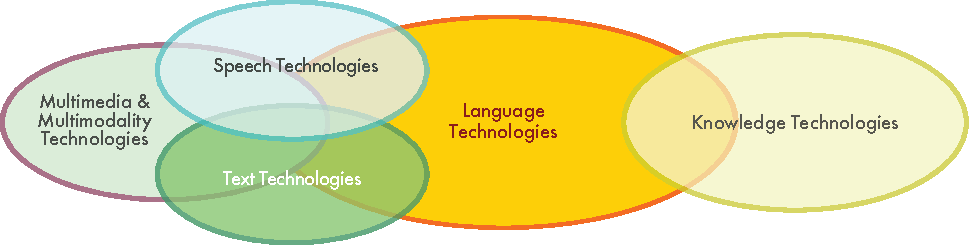
\includegraphics[width=\textwidth]{../_media/english/language_technologies}
  \caption{Language technology in context}
  \label{fig:ltincontext_en}
  \colorrule{grey3}{\textwidth}{1.5pt}
\end{figure*}

When we communicate, we combine language with other modes of communication and information media – for example speaking can involve gestures and facial expressions. Digital texts link to pictures and sounds. Movies may contain language in spoken and written form. In other words, speech and text technologies overlap and interact with other multimodal communication and multimedia technologies.\\ 
In this section, we will discuss the main application areas of language technology, i.\,e., language checking, web search, speech interaction, and machine translation. These applications and basic technologies include the following:

\begin{itemize}
\item spelling correction
\item authoring support
\item computer-assisted language learning
\item information retrieval 
\item information extraction
\item text summarisation
\item question answering
\item speech recognition 
\item speech synthesis 
\end{itemize}

Language technology is an established area of research with an extensive set of introductory literature.
%start Norwegian
The interested reader is referred to textbooks \cite{jurafsky-martin01, manning-schuetze1}, surveys {lt-survey1} and the website LT World (\url{http://www.lt-world.org}).
%end Norwegian

Before discussing the above application areas, we will briefly describe the architecture of a typical LT system.

\subsection{Application Architectures}

Software applications for language processing typically consist of several components that mirror different aspects of language. While such applications are typically very complex, figure~\ref{fig:textprocessingarch_en} shows a highly simplified architecture of a typical text processing system. The first three modules handle the structure and meaning of the text input:

\begin{enumerate}
\item Pre-processing: cleans the data, analyses or removes formatting, detects the input languages, and so on.
\item Grammatical analysis: finds the verb, its objects, modifiers and other parts of speech; detects the sentence structure.
\item Semantic analysis: performs disambiguation (i.\,e., computes the appropriate meaning of words in a given context); resolves anaphora (i.\,e., which pronouns refer to which nouns in the sentence); represents the meaning of the sentence in a machine-readable way.
\end{enumerate}

After analysing the text, task-specific modules can perform other operations, such as automatic summarisation and database look-ups.

In the remainder of this section, we firstly introduce the core application areas for language technology, and follow this with a brief overview of the state of LT research and education today, and a description of past and present research programmes. Finally, we present an expert estimate of core LT tools and resources for German in terms of various dimensions such as availability, maturity and quality. The general situation of LT for the German language is summarised in a matrix (figure~\ref{fig:lrlttable_en}). Tools and resources that are boldfaced in the text can also be found in figure~\ref{fig:lrlttable_en} (p.~\pageref{fig:lrlttable_en}) at the end of this chapter. LT support for German is also compared to other languages that are part of this series.

\begin{figure*}[htb]
  \colorrule{grey3}{\textwidth}{1.5pt}
  \center
  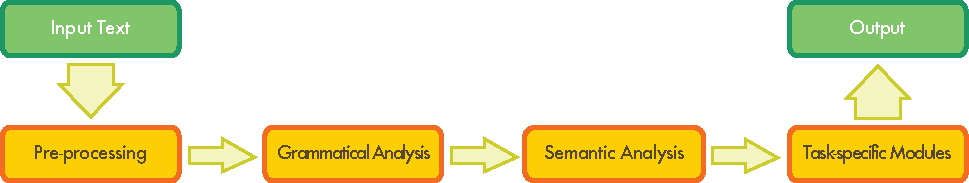
\includegraphics[width=\textwidth]{../_media/english/text_processing_app_architecture}
  \caption{A typical text processing architecture}
  \label{fig:textprocessingarch_en}
  \colorrule{grey3}{\textwidth}{1.5pt}
\end{figure*}

\subsection{Core Application Areas}

In this section, we focus on the most important LT tools and resources, and provide an overview of LT activities in 
%start Norwegian
Norway. 
%end Norwegian

\subsubsection{Language Checking}

Anyone who has used a word processor such as Microsoft Word knows that it has a spell checker that highlights spelling mistakes and proposes corrections. The first spelling correction programs compared a list of extracted words against a dictionary of correctly spelled words. Today these programs are far more sophisticated. Using language-dependent algorithms for \textbf{grammatical analysis}, they detect errors related to morphology (e.\,g., plural formation) as well as syntax–related errors, such as a missing verb or a conflict of verb-subject agreement (e.\,g., \textit{she *write a letter}). However, most spell checkers will not find any errors in the following text \cite{zar1}:

\begin{quote}
  I have a spelling checker,\\
  It came with my PC.\\
  It plane lee marks four my revue\\
  Miss steaks aye can knot sea.
\end{quote}

%start Norwegian
Handling these kinds of errors usually requires an analysis of the context, for example to decide if a Norwegian word should be spelled with one or with a double consonant in Norwegian, as in \textit{vil} (will, would like to) vs. \textit{vill} (wild].

This type of analysis either needs to draw on language-specific grammars, laboriously coded into the software by experts, or on a statistical language model. The latter calculates the probability of a particular word as it occurs in a specific position (e.\,g., between the words that precede and follow it). For example, \textit{jeg vil ha} (I would like to have) is a much more probable word sequence than \textit{jeg vill ha} (I wild have). A statistical language model can be automatically created by using a large amount of (correct) language data, a \textbf{text corpus}.

Implementations of these two approaches have been developed around data from English. Neither approach can transfer easily to Norwegian with its different word order, compound building and richer inflection for certain word classes than in English, and studies for Norwegian are therefore needed. Furthermore, due to the particularity that Norwegian has two official written norms, one of which is lesser used, the need for good proofing tools for each written norm is significant. 
%end Norwegian

\begin{figure*}[htb]
  \colorrule{grey3}{\textwidth}{1.5pt}
  \center
  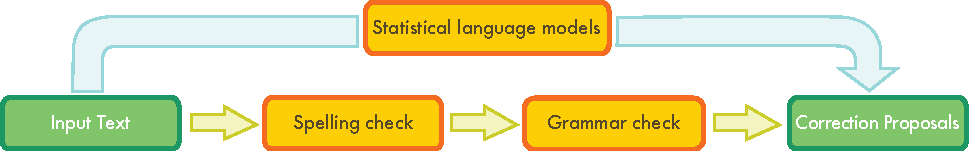
\includegraphics[width=\textwidth]{../_media/english/language_checking}
  \caption{Language checking (statistical; rule-based)}
  \label{fig:langcheckingaarch_en}
  \colorrule{grey3}{\textwidth}{1.5pt}
\end{figure*}

Language checking is not limited to word processors; it is also used in \textbf{authoring support systems}, i.\,e., software environments in which manuals and other types of technical documentation for complex IT, healthcare, engineering and other products, are written. To offset customer complaints about incorrect use and damage claims resulting from poorly understood instructions, companies are increasingly focusing on the quality of technical documentation while targeting the international market (via translation or localisation) at the same time. Advances in natural language processing have led to the development of authoring support software, which helps the writer of technical documentation to use vocabulary and sentence structures that are consistent with industry rules and (corporate) terminology restrictions.

\boxtext{The use of language checking is not limited to word processors. It also applies to authoring support systems.}

%start Norwegian
Adequate spell checkers would provide an important tool to alleviate the writing process for individuals with writing difficulties, be it dyslectics or second language learners, since a context sensitive analysis may enable fewer and more relevant spelling suggestions: many choices demand a high level of reading ability and linguistic awareness.

Some Norwegian companies and language service providers develop products in the area of language checking. 
On the research side, basic LT resources that may be of use for Language Checking (lexicons, word lists, text corpora, compound analyzers) are developed mainly at the University of Oslo, the University of Bergen and Uni Research in Bergen. 

The most widely used proofing tool for Norwegian, the one found in the Microsoft Office suite, is made by the Finnish company Lingsoft, while parts of its grammar checker for Bokmål were developed by researchers at the University of Oslo. 
Spell checking for Bokmål and Nynorsk using open source technologies such as \textit{Hunspell} are also available.
Another Norwegian commercial actor is Tansa, which specializes in text proofing tools that are tuned to the specific needs and vocabularies of individual larger enterprises. 
Covering several languages in addition to Norwegian Bokmål and Nynorsk (e.g. English, German, Spanish and French) their customers range from the Norwegian Broadcasting Corporation NRK to the Financial Times. 
Nynodata AS offers a writing aid tool from Bokmål to Nynorsk which translates and also ensures that the resulting word inflections adheres to the user’s chosen writing norm.

Three companies specifically target writing aid tools for dyslectics. 
Two of them, Lingit and Include, include a spell checker component as well as other reading and writing aid tools (word prediction, text-to-speech components), while MikroVerkstedet includes word completion and word prediction components.

On the face of it, the situation for Norwegian proofing tools may seem quite encouraging. 
But at the same time, several of the initiatives are quite fragile. 
For instance, Norwegian spell checking based on open source technologies (\textit{aspell, Hunspell}) is maintained by three individuals who use their spare time to do so. 
One may say that one of the major competitors to Microsoft software on the Norwegian market hinges on the personal initiatives of a few dedicated individuals rather than a systematic effort towards the development of open source modules. Moreover, a significant challenge for most Norwegian proofing tools is to \textit{improve} the existing basic resources by developing more advanced Language Technology tools. Finally, language specific tools for the automatic translation or translation support of Norwegian are missing. Translation memory tools such as Trados exist, but they do not contain language specific adjustment for Norwegian beyond basic spell checking.

Besides spell checkers and authoring support, language checking is also important in the field of computer-assisted language learning. Language checking applications also automatically correct search engine queries, as found in Google's \textit{Did you mean…} suggestions.
%end Norwegian

\subsubsection{Web Search}

\begin{figure*}[htb]
  \colorrule{grey3}{\textwidth}{1.5pt}
  \center
  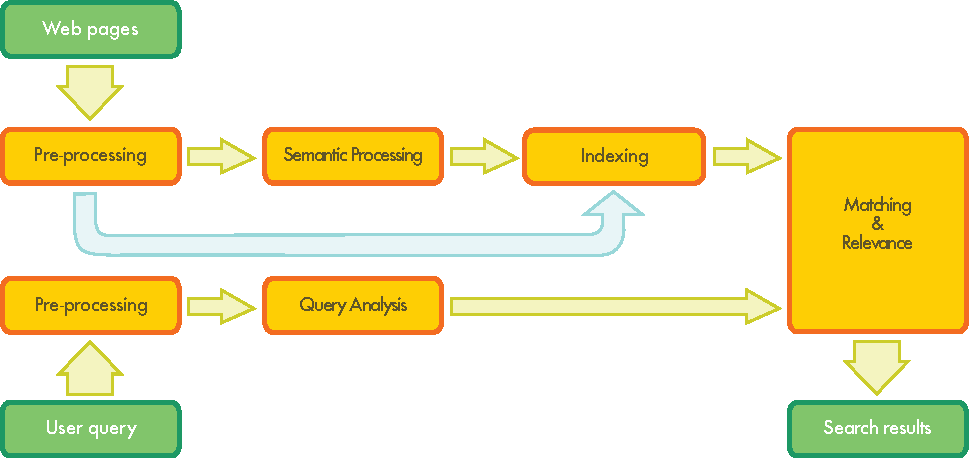
\includegraphics[width=\textwidth]{../_media/english/web_search_architecture}
  \caption{Web search}
  \label{fig:websearcharch_en}
  \colorrule{grey3}{\textwidth}{1.5pt}
 \end{figure*}

Searching the Web, intranets or digital libraries is probably the most widely used yet largely underdeveloped language technology application today. The Google search engine, which started in 1998, now handles about 80\% of all search queries \cite{spi1}. 
The Google search interface and results page display has not significantly changed since the first version. However, in the current version, Google offers spelling correction for misspelled words and incorporates basic semantic search capabilities that can improve search accuracy by analysing the meaning of terms in a search query context \cite{pc1}. The Google success story shows that a large volume of data and efficient indexing techniques can deliver satisfactory results using a statistical approach to language processing. 

For more sophisticated information requests, it is essential to integrate deeper linguistic knowledge to facilitate text interpretation. Experiments using lexical resources such as machine-readable thesauri or ontologies
%start Norwegian
(a Norwegian wordnet is expected by the end of 2012)
%end Norwegian
have demonstrated improvements in finding pages using synonyms of the original search terms, such as
\textit{atomkraft} (atomic energy), \textit{kjerneenergi} (atomic power) and \textit{nukleærenergi} (nuclear energy),
or even more loosely related terms.

\boxtext{The next generation of search engines will have to include much more sophisticated language technology.}

The next generation of search engines will have to include much more sophisticated language technology, escpecially to deal with search queries consisting of a question or other sentence type rather than a list of keywords. For the query \textit{Give me a list of all companies that were taken over by other companies in the last five years}, a syntactic as well as \textbf{semantic analysis} is required. The system also needs to provide an index to quickly retrieve relevant documents. A satisfactory answer will require syntactic parsing to analyse the grammatical structure of the sentence and determine that the user wants companies that have been acquired, rather than companies that have acquired other companies. For the expression \textit{last five years}, the system needs to determine the relevant range of years, taking into account the present year. The query then needs to be matched against a huge amount of unstructured data to find the pieces of information that are relevant to the user’s request. This process is called information retrieval, and involves searching and ranking relevant documents. To generate a list of companies, the system also needs to recognise a particular string of words in a document represents a company name, using a process called named entity recognition.

A more demanding challenge is matching a query in one language with documents in another language. Cross-lingual information retrieval involves automatically translating the query into all possible source languages and then translating the results back into the user's target language.

Now that data is increasingly found in non-textual formats, there is a need for services that deliver multimedia information retrieval by searching images, audio files and video data. In the case of audio and video files, a speech recognition module must convert the speech content into text (or into a phonetic representation) that can then be matched against a user query.

%start Norwegian
In Norway, Opera Software developed the first Norwegian web browser and Internet suite.
Opera began in 1994 as a research project within Norway’s largest telecom company, Telenor. 
Within a year, it demerged into an independent development company named Opera Software ASA.
A few companies develop or apply search solutions (CognIT, Comperio, TextUrgy, Abtrox and Infofinder). 
FAST developed a search engine, which was then bought by Microsoft, and which is now being traded by Comperio. 
The development focus for these companies lies on providing add-ons and advanced search engines by exploiting topic-relevant semantics. 
Thus, one may say that the IT industry in Norway already has quite a good foundation as regards web search and information retrieval; the main need reported from the companies is that of reliable LRT components.
%end Norwegian

\subsubsection{Speech Interaction}

Speech interaction is one of many application areas that depend on speech technology, i.\,e., technologies for processing spoken language. Speech interaction technology is used to create interfaces that enable users to interact in spoken language instead of using a graphical display, keyboard and mouse.  Today, these voice user interfaces (VUI) are used for partially or fully automated telephone services provided by companies to customers, employees or partners. Business domains that rely heavily on VUIs include banking, supply chain, public transportation, and telecommunications. Other uses of speech interaction technology include interfaces to car navigation systems and the use of spoken language as an alternative to the graphical or touchscreen interfaces in smartphones.

\begin{figure*}[htb]
  \colorrule{grey3}{\textwidth}{1.5pt}
  \center
  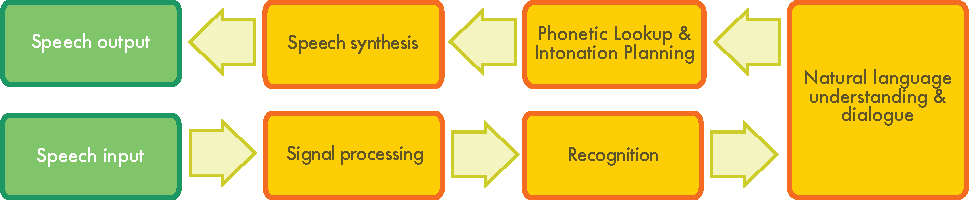
\includegraphics[width=\textwidth]{../_media/english/simple_speech-based_dialogue_architecture}
  \caption{Speech-based dialogue system}
  \label{fig:dialoguearch_en}
  \colorrule{grey3}{\textwidth}{1.5pt}
\end{figure*}

Speech interaction technology comprises four technologies: 

\begin{enumerate}
\item Automatic \textbf{speech recognition} (ASR) determines which words are actually spoken in a given sequence of sounds uttered by a user.  
\item Natural language understanding analyses the syntactic structure of a user’s utterance and interprets it according to the system in question.
\item Dialogue management determines which action to take given the user input and system functionality.   
\item \textbf{Speech synthesis} (text-to-speech or TTS) transforms the system’s reply into sounds for the user.
\end{enumerate}

One of the major challenges of ASR systems is to accurately recognise the words a user utters. This means restricting the range of possible user utterances to a limited set of keywords, or manually creating language models that cover a large range of natural language utterances. Using machine learning techniques, language models can also be generated automatically from \textbf{speech corpora}, i.\,e., large collections of speech audio files and text transcriptions. Restricting utterances usually forces people to use the voice user interface in a rigid way and can damage user acceptance; but the creation, tuning and maintenance of rich language models will significantly increase costs. VUIs that employ language models and initially allow a user to express their intent more flexibly -- prompted by a \textit{How may I help you?} greeting -- tend to be automated and are better accepted by users.

\boxtext{Speech interaction is the basis for creating interfaces that allow a user to interact with spoken language instead of a graphical display, keyboard and mouse.}

Companies tend to use pre-recorded utterances by professional speakers for generating the output of the voice user interface. For static utterances where the wording does not depend on particular contexts of use or personal user data, this can deliver a rich user experience. But more dynamic content in an utterance may suffer from unnatural intonation because bits of audio files have simply been strung together. Through optimisation, today’s TTS systems are getting better at producing natural-sounding dynamic utterances.

Interfaces in speech interaction have been considerably standardised during the last decade in terms of their various technological components. There has also been strong market consolidation in speech recognition and speech synthesis. The national markets in the G20 countries (economically resilient countries with high populations) have been dominated by just five global players, with Nuance (USA) and Loquendo (Italy) being the most prominent players in Europe. In 2011, Nuance announced the acquisition of Loquendo, which represents a further step in market consolidation.

%start Norwegian
In the Norwegian TTS market, thirteen Norwegian voices of varying quality are available, some of which have been developed by the above mentioned European players. 
Three voices have been developed by the Norwegian company Lingit, which targets users groups with reading and writing impairments. 
Another voice was developed by the Norwegian Library of Talking Books and Braille in cooperation with their sister library in Sweden. 
There is also an active research community at Norwegian University of Science and Technology in Trondheim. 
The quality of speech synthesis depends heavily on available resources (in particular text corpora tagged for part of speech, tokenizers and pronunciation lexicons) and language specific research on for instance prosodic features for the language in question. 
Such resources are abundant for English but only to a lesser extent for Norwegian, even if Norwegian is especially challenging due to the wide variety of possible spelling variants and the range of dialects; moreover the tonal accents in most Norwegian dialects and the lack of a one-to-one relation between sounds and letters pose challenges.

Regarding dialogue management technology and know-how, the market is rather dominated by national, smaller enterprises. 
MediaLT has developed a general speech recognition engine used for dialogue management for the visually impaired. 
Regarding speech-to-text, Max Manus has integrated and localised Philips’ SpeechMagic for Norwegian hospitals. 
This system is relatively successful, but it is limited to a relatively closed domain (with a closed vocabulary). 
Recently Dragon Dictation, a voice recognition application for mobile telephones, was launched for Norwegian. 
This application is the first \textit{general} dictation system for Norwegian; however the Norwegian version of Dragon Dictation seems to misinterpret conspicuously more than the English counterpart.
Within the domain of speech interaction, a genuine market for the linguistic core technologies for syntactic and semantic analysis does not exist yet.
%end Norwegian

Looking ahead, there will be significant changes, due to the spread of smartphones as a new platform for managing customer relationships, in addition to fixed telephones, the Internet and e-mail. This will also affect how speech interaction technology is used. In the long term, there will be fewer telephone-based VUIs, and spoken language apps will play a far more central role as a user-friendly input for smartphones. This will be largely driven by stepwise improvements in the accuracy of speaker-independent speech recognition via the speech dictation services already offered as centralised services to smartphone users.

\subsubsection{Machine Translation}

\begin{figure*}[htb]
  \colorrule{grey3}{\textwidth}{1.5pt}
  \center
  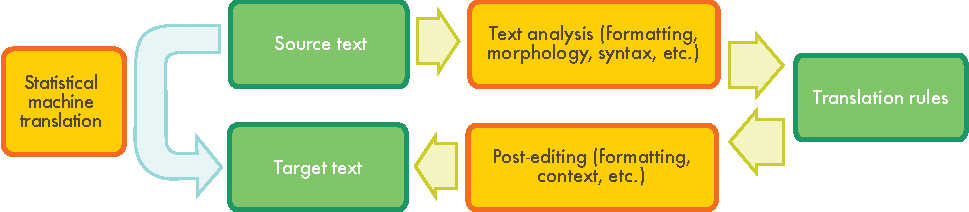
\includegraphics[width=\textwidth]{../_media/english/machine_translation}
  \caption{Machine translation (statistical / rule-based)}
  \label{fig:mtarch_en}
  \colorrule{grey3}{\textwidth}{1.5pt}
\end{figure*}

The idea of using digital computers to translate natural languages can be traced back to 1946 and was followed by substantial funding for research during the 1950s and again in the 1980s. 
Yet \textbf{machine translation} (MT) still cannot deliver on its initial promise of providing across-the-board automated translation.  

\boxtext{At its basic level, Machine Translation simply substitutes words in one natural language with words in another language.}

The most basic approach to machine translation is the automatic replacement of the words in a text written in one natural language with the equivalent words of another language. This can be useful in subject domains that have a very restricted, formulaic language such as weather reports.
However, in order to produce a good translation of less restricted texts, larger text units (phrases, sentences, or even whole passages) need to be matched to their closest counterparts in the target language. The major difficulty is that human language is ambiguous.

%start Norwegian
Ambiguity creates challenges on multiple levels, such as word sense disambiguation on the lexical level or syntactic ambiguities at the sentence level. 
A likely idiomatic translation of the Norwegian sentence \textit{\bokmaal{Plutselig røk slangen}\nynorsk{Plutseleg rauk slangen}} in English could be \textit{Suddenly the hose snapped.}
However, a simple word-by-word translation of this sentence might yield \textit{Suddenly smoked the snake.}
This is because the verb form \textit{\bokmaal{røk}\nynorsk{rauk}} (past tense of \textit{ryke}) is ambiguous between `snap' and `smoke' whereas \textit{slange} is ambiguous between `hose' and `snake'; note also that a simple word-by-word translation would not get the difference in word order between Norwegian and English right.

In addition to lexical ambiguities and word order differences, another challenge is syntactic ambiguities. 
In Norwegian we may topicalize objects, but this possibility is much more restricted in English. 
The Norwegian sentence \textit{\bokmaal{Eplene}\nynorsk{epla} spiste mannen} has two possible interpretations: either \textit{\bokmaal{Eplene}\nynorsk{epla}} (the apples) is analysed as the subject of the sentence (the apples ate the man) or as a topicalized object (the apples were eaten by the man). 
Since this ambiguity does not exist in English, a machine translation system must first identify the correct syntactic interpretation in order to find the correct translation. 

Another MT challenge for Norwegian is compounding. 
An efficient translation system must thus be able to discover newly coined compounds, resolve them, and, if needed, create new compounds in the target language. 
%end Norwegian

For translations between closely related languages, a translation using direct substitution may be feasible for many sentences. However, rule-based (or linguistic knowledge-driven) systems often analyse the input text and create an intermediary symbolic representation from which the target language text can be generated. The success of these methods is highly dependent on the availability of extensive lexicons with morphological, syntactic, and semantic information, and large sets of grammar rules carefully designed by skilled linguists. This is a very long and therefore costly process.

In the late 1980s when computational power increased and became cheaper, interest in statistical models for machine translation began to grow. Statistical models are derived from analysing bilingual text corpora, \textbf{parallel corpora}, such as the Europarl parallel corpus, which contains the proceedings of the European Parliament in 11 European languages
%start Norwegian
(Norwegian not being one of them).
%end Norwegian
Given enough data, statistical MT works well enough to derive an approximate meaning of a foreign language text by processing parallel versions and finding plausible patterns of words. Unlike knowledge-driven systems, however, statistical (or data-driven) MT systems often generate ungrammatical output. Data-driven MT is advantageous because less human effort is required, and it can also cover special particularities of the language (e.\,g., idiomatic expressions) that are often ignored in knowledge-driven systems. 

The strengths and weaknesses of knowledge-driven and data-driven machine translation tend to be complementary, so that nowadays researchers focus on hybrid approaches that combine both methodologies. One such approach uses both knowledge-driven and data-driven systems, together with a selection module that decides on the best output for each sentence. However, results for sentences longer than, say, 12 words, will often be far from perfect. A more effective solution is to combine the best parts of each sentence from multiple outputs; this can be fairly complex, as corresponding parts of multiple alternatives are not always obvious and need to be aligned. 

\boxtext{Although the need for Machine Translation for Norwegian is apparent, the development of such software for Norwegian is not extensive.}

Two systems address the fact that Norwegian has two written norms, creating a need for efficient translations between the written norms. 
The small enterprise Nynodata offers tools for translation, correction and text search for Bokmål and Nynorsk. 
The open-source initiative Apertium also offers automated translation between the two written norms, implemented by a student at the University of Bergen. 

Google Translate has a Norwegian module to translate between English and Norwegian, and via English it is possible to translate between Norwegian and any language pair containing English. 
GramTrans is an MT platform developed in cooperation between the Danish GrammarSoft ApS and the Norwegian company Kaldera Språkteknologi AS. 
The translation engine offers free web-based translation for the Scandinavian languages and also between Norwegian and English, based on a robust grammatical analysis, a transfer component for lexicon and grammar and a generation component. 
The company Clue Norge, which specialises in electronic dictionaries for enterprises, developed a system (Textran) for machine translation from English to Norwegian about ten years ago. 
The system still exists but was not further developed because perfect translations are hard to obtain whereas the user groups were not ready to pay for a less than perfect system.

Although significant research in this technology exists in national and international contexts, data-driven and hybrid systems have so far been less successful in business applications than in the research lab. 
In Norway, the main research expertise in this field is found at the University of Oslo and the University of Bergen.

The use of machine translation can significantly increase productivity provided the system is intelligently adapted to user-specific terminology and integrated into a workflow. 
In general, there seems to be an underuse of language technology resources in the Norwegian Language Service Industry. 
This sector can be divided into two groups: on the one hand there are freelance translators and translation agencies catering to individual clients, commercial actors and the public sector, and on the other hand there are translators affiliated with \textit{Oversetterforeningen} (Organisation of translators of literary texts) and \textit{Norsk faglitterær forfatter- og oversetterforening} (Organization of translators of scientific and academic texts). 

In the latter group, the use of language technology is limited. 
The former group uses Trados, which is the dominant machine translation tool for professional translators. 
However, Trados has no Norwegian module but is based on Hunspell, an open source spell checker and morphological analyzer originally developed for Hungarian which is not optimal for Norwegian. 
Although it is a functional and open solution, it still needs further development to be an optimal resource for the Norwegian Language Service industry and there is a particular need for improvement of the analysis of Norwegian compounds. 

In addition, professional translators use term bases (UD, IATE) and to some extent collaborate with the University Sector in developing term base resources. 
The apparent underuse of language technology resources in the Language Service Industry is caused in part by the lack of adequate resources for Norwegian, but also by a lacking contact between the Language Service Industry and the research community. 
As a consequence, knowledge of the full spectrum of language technology is often too limited, and it is difficult for commercial actors to evaluate the quality of a resource. 
%end Norwegian

There is still a huge potential for improving the quality of MT systems. The challenges involve adapting language resources to a given subject domain or user area, and integrating the technology into workflows that already have term bases and translation memories. Another problem is that most of the current systems are English-centred and only support a few languages from and into German. This leads to friction in the translation workflow and forces MT users to learn different lexicon coding tools for different systems.

Evaluation campaigns help to compare the quality of MT systems, the different approaches and the status of the systems for different language pairs.
%start Norwegian
The EuroMatrixPlus project carried out a survey of machine translation performance between 22 official EU languages.
Norwegian was not included in this project.
%end Norwegian

\subsection{Other Application Areas}

Building language technology applications involves a range of subtasks that do not always surface at the level of interaction with the user, but they provide significant service functionalities `behind the scenes' of the system in question. They all form important research issues that have now evolved into individual sub-disciplines of computational linguistics.  Question answering, for example, is an active area of research for which annotated corpora have been built and scientific competitions have been initiated. The concept of question answering goes beyond keyword-based searches (in which the search engine responds by delivering a collection of potentially relevant documents) and enables users to ask a concrete question to which the system provides a single answer. For example:

\begin{quote}
Question: \textit{How old was Neil Armstrong when he stepped on the moon?}\\
Answer: \textit{38.}
\end{quote}

While question answering is obviously related to the core area of web search, it is nowadays an umbrella term for such research issues as which different types of questions exist, and how they should be handled; how a set of documents that potentially contain the answer can be analysed and compared (do they provide conflicting answers?); and how specific information (the answer) can be reliably extracted from a document without ignoring the context. 

\boxtext{Language technology applications often provide significant service functionalities `behind the scenes' of larger software systems.}

Question answering is in turn related to information extraction (IE), an area that was extremely popular and influential when computational linguistics took a statistical turn in the early 1990s. IE aims to identify specific pieces of information in specific classes of documents, such as the key players in company takeovers as reported in newspaper stories. Another common scenario that has been studied is reports on terrorist incidents. The task here consists of mapping appropriate parts of the text to a template that specifies the perpetrator, target, time, location and results of the incident. Domain-specific template-filling is the central characteristic of IE, which makes it another example of a `behind the scenes' technology that forms a well-demarcated research area, which in practice needs to be embedded into a suitable application environment. 

    \textbf{Text summarisation} and \textbf{text generation} are two borderline areas that can act either as standalone applications or play a supporting role. Summarisation attempts to give the essentials of a long text in a short form, and is one of the features available in Microsoft Word. It mostly uses a statistical approach to identify the `important' words in a text (i.\,e., words that occur very frequently in the text in question but less frequently in general language use) and determine which sentences contain the most of these `important' words. These sentences are then extracted and put together to create the summary. In this very common commercial scenario, summarisation is simply a form of sentence extraction, and the text is reduced to a subset of its sentences. An alternative approach, for which some research has been carried out, is to generate brand new sentences that do not exist in the source text. 

%start Norwegian
\boxtext{For the Norwegian language, research in most text technologies is much less developed than for the English language.}

This requires a deeper understanding of the text, which means that so far this approach is far less robust. On the whole, a text generator is rarely used as a stand-alone application but is embedded into a larger software environment, such as a clinical information system that collects, stores and processes patient data. Creating reports is just one of many applications for text summarisation.

Question answering, information extraction, and summarisation have been the focus of numerous open competitions in the USA since the 1990s, primarily organised by the government-sponsored organisations DARPA and NIST. 
These competitions have significantly improved the start-of-the-art, but their focus has mostly been on the English language. 
As a result, there are hardly any annotated corpora or other special resources needed to perform these tasks in Norwegian. 
When summarisation systems use purely statistical methods, they are largely language-independent and a number of research prototypes are available. 
For text generation, reusable components have traditionally been limited to surface realization modules (generation grammars) and most of the available software is for the English language.
%end Norwegian

\subsection{Educational Programmes}

Language technology is a very interdisciplinary field that involves the combined expertise of linguists, computer scientists, mathematicians, philosophers, psycholinguists, and neuroscientists among others. 
%start Norwegian
As a result, it has not acquired a clear, independent existence in the Norwegian higher education system. 

In Norway, scientific expertise is present in small research groups at the universities of Oslo, Bergen, and Tromsø, the Norwegian University of Science and Technology, the Norwegian School of Economics and the research companies Uni Research and Sintef) that cooperate on a project basis. 
No universities have established separate departments or centres of Computational Linguistics or Language Technology. 
%GIL: fjernet fra følgende originalsetning at datalingvistikkundervisning foregår BÅDE ved lingvistikk/UiO og infirmatikk/UiO: A limited number of relevant courses are offered by departments of Computer Science (University of Oslo and Norwegian University of Science and Technology) and Linguistics (Universities of Bergen, Oslo and Tromsø). 
A limited number of relevant courses are offered by departments of Computer Science (University of Oslo and Norwegian University of Science and Technology) and Linguistics (Universities of Bergen and Tromsø). 
Research and teaching in speech processing is only represented at the Norwegian University of Science and Technology. 

Although it is hard to quantify such a claim, the field of Computational Linguistics, and the options to study it, do not appear to be very well-known in Norway. 
Indeed, a crux of the KUNSTI programme was to strengthen basic research and the competence within language technology disciplines. %\footnote{http://www.forskningsradet.no/servlet/Satellite?c=Page\&pagename=kunsti\%2FHovedsidemal\&cid=1232959399366}. 
%KUNSTI \footnote{http://www.forskningsradet.no/servlet/Satellite?c=Page\&cid=1232959399409\&pagename=kunsti\%2FHovedsidemal}
This program enabled several master's and PhD theses to be completed in relation to the wide variety of research projects. 
One may therefore say that this program was instrumental in stimulating a framework to foster new researchers and a wider competence in LRT for Norwegian.

The University of Bergen coordinates CLARA, a Marie Curie Initial Training Network aimed at offering researcher training in LRT at nine European facilities.

\subsection{National Projects and Initiatives}

Since the Norwegian language industry is relatively small by international standards, national and local academic initiatives have been important for the development of Norwegian LRT, also for the benefit of private companies.
Most Norwegian companies in need of LRT express their desire to take advantage of resources, knowledge and expertise in academia, because their own main expertise usually does not lie in LRT.

The Research Council of Norway has supported one language technology research program, namely KUNSTI (Kunnskapsutvikling for norsk språkteknologi).
It was in part inspired by larger projects in other countries (e.g. the German project Verbmobil) and aimed to increase competence in language technology through basic research. 
KUNSTI aimed for R\&D to make spoken and written Norwegian in various forms (and to some extent Saami) accessible for computer processing. 
Twenty research projects of varying sizes were completed under the program, the largest two being in MT and speech processing.

Building a variety of language technology applications presupposes basic resources, such as word lists, text corpora and speech corpora. 
These are just as costly and time-consuming to develop for smaller languages as for larger languages; since Norwegian has two official written norms, the costs are even higher. 
Therefore, Norwegian is not very attractive from a commercial point of view. 

It is for this reason that it was such an important achievement to establish the \textit{Language Technology Resource Collection for Norwegian -- Språkbanken} in 2010, after two decades of joint efforts between the Norwegian Language Council, the Research Council, commercial companies and the Norwegian research institutions. 
Språkbanken at the National Library is to function as an infrastructure for making Norwegian LRT available for research and commercial use, thus hopefully reducing the threshold for developing Norwegian LRT products. 

The situation thus far has been that whereas private companies compile various in-house resources and tools, substantial resources and tools, for instance lexicons, taggers and named-entity recognizers, are developed at research institutions and is subsequently sometimes purchased in some form by private companies. 
Indeed, the majority of tools and resources listed in the Table of Tools and Resources at the end of this report are developed at the research institutions. 
For instance, the University of Oslo has developed the speech corpora NoTa-Oslo (Norsk Talespråkskorpus, the Oslo part) and Nordic Dialect Corpus, Norsk Ordbank has been developed by the University of Oslo in cooperation with the Norwegian Language Council, the Oslo-Bergen tagger has been made by the University of Oslo and Uni Research in Bergen, the Norwegian Newspaper Corpus has been developed by Uni Research and the Norwegian School of Economics and the INESS treebanking infrastructure is currently being built at the University of Bergen.

In the work program of KUNSTI, the development of basic language and speech data was not catered for. 
It was therefore felt that the projects under this programme were hampered by a lack of basic language resources. 
With Språkbanken now established, and with new researchers and revitalized competence, it is felt by many that the time may be ripe to consider a new LRT effort which may get a more application-oriented focus than its predecessor. 

Sizeable LRT building projects (e.g. the INESS, NoTa-Oslo (Norsk Talespråkskorpus, the Oslo part), Norsk aviskorpus, WeSearch—Language technology for the web and SIRKUS) after KUNSTI have been financed through infrastructure programs (AVIT) or general ICT programs from the Research Council such as VERDIKT. 
As a part of building basic Norwegian LRT, Språkbanken signed a contract with Kaldera språkteknologi AS in 2011 to create wordnets for Norwegian. % Bokmål and Nynorsk. %\footnote{http://www.nb.no/spraakbanken/english/projects}. 
Public funding for LT projects in Norway and in Europe is still relatively low, however, when compared to the amount of money the USA spends on language translation and multilingual information access \cite{laz1}.

As we have seen, previous programmes have led to the development of a number of LT tools and resources for the Norwegian language. 

In the following section, the current state of LT support for Norwegian is summarised.
  
\subsection{Availability of Tools and Resources}

Figure~\ref{fig:lrlttable_en} provides a rating for language technology support for Norwegian. This rating of existing tools and resources was generated by leading experts in the field who provided estimates based on a scale from 0 (very low) to 6 (very high) using seven criteria.

%the following table needs numbers for Norwegian
\begin{figure*}[htb]
\centering
%\begin{tabular}{>{\columncolor{orange1}}p{.33\linewidth}ccccccc} % ORIGINAL
\begin{tabular}{>{\columncolor{orange1}}p{.33\linewidth}@{\hspace*{6mm}}c@{\hspace*{6mm}}c@{\hspace*{6mm}}c@{\hspace*{6mm}}c@{\hspace*{6mm}}c@{\hspace*{6mm}}c@{\hspace*{6mm}}c}
\rowcolor{orange1}
 \cellcolor{white}&\begin{sideways}\makecell[l]{Quantity}\end{sideways}
&\begin{sideways}\makecell[l]{\makecell[l]{Availability} }\end{sideways} &\begin{sideways}\makecell[l]{Quality}\end{sideways}
&\begin{sideways}\makecell[l]{Coverage}\end{sideways} &\begin{sideways}\makecell[l]{Maturity}\end{sideways} &\begin{sideways}\makecell[l]{Sustainability}\end{sideways} &\begin{sideways}\makecell[l]{Adaptability}\end{sideways} \\ \addlinespace
\multicolumn{8}{>{\columncolor{orange2}}l}{Language Technology: Tools, Technologies and Applications} \\ \addlinespace
Speech Recognition &4&2&2&1&2&3&3 \\ \addlinespace
Speech Synthesis &3&2&3&2&3&3&3\\ \addlinespace
Grammatical analysis &4&4,5&4&4&4,5&4,5&5\\ \addlinespace 
Semantic analysis &2&2&3,3&3&3,7&3,3&3,7\\ \addlinespace
Text generation &1&4&4&3&5&4&5\\ \addlinespace
Machine translation &4&4&2&2&3&5&3\\ \addlinespace
\multicolumn{8}{>{\columncolor{orange2}}l}{Language Resources: Resources, Data and Knowledge Bases} \\ \addlinespace
Text corpora &4,5&3,5&3,5&3&4&4,5&4\\ \addlinespace
Speech corpora &5&4&3&5&4&5&5\\ \addlinespace
Parallel corpora &5&3&2&2&4&3&3\\ \addlinespace
Lexical resources &2,5&2&2&2&2&2&2,5\\ \addlinespace
Grammars &2&4&5&3&4&5&3\\
\end{tabular}
\caption{State of language technology support for Norwegian}
\label{fig:lrlttable_en}
\end{figure*}

The key results for Norwegian language technology can be summed up as follows:

\begin{itemize}
\item Norwegian stands reasonably well with respect to the most basic language technology tools and resources, such as tokenizers, PoS taggers, morphological analysers, reference corpora, and speech corpora. 
There are also many speech synthesis (TTS) products for Norwegian with a general applicability and an acceptable quality, although most of them are developed by commercial actors and are thus restricted in terms of availability. Lexicons covering general language are well-represented but there are major gaps in the coverage of terminologies representing specialized domains.
\item Individual products with limited functionality exist in subfields such as speech recognition, machine translation, text semantics and a few others. 
Some of these areas are covered for Norwegian by commercial actors and are thus restricted in terms of availability.
\item Some tools and resources are virtually non-existing; furthermore some resources are developed for commercial use and are not available. 
This typically applies to tools and resources for more advanced Norwegian language technology such as a advanced discourse processing, text generation and ontologies for representing world knowledge.
\item At present, many of the tools and resources lack standardisation, i.e., even if they exist, sustainability and adaptability are not necessarily catered for. 
Although the table suggests that basic LT tools and resources exist for Norwegian, they are in some cases fragmented and their sustainability is limited by restrictions on their use, incompatibilities and insufficient documentation. 
\end{itemize}

To conclude, today we have software with limited functionality available in a number of specific areas of Norwegian language research. 
Obviously, further research efforts are required to meet the current deficit in processing texts on a deeper semantic level and to address the lack of resources such as parallel corpora for machine translation.
%end Norwegian

\subsection{Cross-language comparison}

\begin{figure*}[tb]
  \small
  \centering
  \begin{tabular}
  { % defines color for each column.
  >{\columncolor{corange5}}p{.13\linewidth}@{\hspace{.040\linewidth}}
  >{\columncolor{corange4}}p{.13\linewidth}@{\hspace{.040\linewidth}}
  >{\columncolor{corange3}}p{.13\linewidth}@{\hspace{.040\linewidth}}
  >{\columncolor{corange2}}p{.13\linewidth}@{\hspace{.040\linewidth}}
  >{\columncolor{corange1}}p{.13\linewidth} 
  }
  \multicolumn{1}{>{\columncolor{white}}c@{\hspace{.040\linewidth}}}{\textbf{Excellent}} & 
  \multicolumn{1}{@{}>{\columncolor{white}}c@{\hspace{.040\linewidth}}}{\textbf{Good}} &
  \multicolumn{1}{@{}>{\columncolor{white}}c@{\hspace{.040\linewidth}}}{\textbf{Moderate}} &
  \multicolumn{1}{@{}>{\columncolor{white}}c@{\hspace{.040\linewidth}}}{\textbf{Fragmentary}} &
  \multicolumn{1}{@{}>{\columncolor{white}}c}{\textbf{Weak/no}} \\ 
  \multicolumn{1}{>{\columncolor{white}}c@{\hspace{.040\linewidth}}}{\textbf{support}} & 
  \multicolumn{1}{@{}>{\columncolor{white}}c@{\hspace{.040\linewidth}}}{\textbf{support}} &
  \multicolumn{1}{@{}>{\columncolor{white}}c@{\hspace{.040\linewidth}}}{\textbf{support}} &
  \multicolumn{1}{@{}>{\columncolor{white}}c@{\hspace{.040\linewidth}}}{\textbf{support}} &
  \multicolumn{1}{@{}>{\columncolor{white}}c}{\textbf{support}} \\ \addlinespace
  
& \vspace*{0.5mm}English
& \vspace*{0.5mm}
Czech \newline 
Dutch \newline 
Finnish \newline 
French \newline 
German \newline   
Italian \newline  
Portuguese \newline 
Spanish \newline
& \vspace*{0.5mm}Basque \newline 
Bulgarian \newline 
Catalan \newline 
Danish \newline 
Estonian \newline 
Galician\newline 
Greek \newline  
Hungarian  \newline
Irish \newline  
Norwegian \newline 
Polish \newline 
Serbian \newline 
Slovak \newline 
Slovene \newline 
Swedish \newline
& \vspace*{0.5mm}
Croatian \newline 
Icelandic \newline  
Latvian \newline 
Lithuanian \newline 
Maltese \newline 
Romanian\\
\end{tabular}
\caption{Speech processing: state of language technology support for 30 European languages}
\label{fig:speech_cluster_en}
\end{figure*}

\begin{figure*}[tb]
  \small
  \centering
  \begin{tabular}
  { % defines color for each column.
  >{\columncolor{corange5}}p{.13\linewidth}@{\hspace{.040\linewidth}}
  >{\columncolor{corange4}}p{.13\linewidth}@{\hspace{.040\linewidth}}
  >{\columncolor{corange3}}p{.13\linewidth}@{\hspace{.040\linewidth}}
  >{\columncolor{corange2}}p{.13\linewidth}@{\hspace{.040\linewidth}}
  >{\columncolor{corange1}}p{.13\linewidth} 
  }
  \multicolumn{1}{>{\columncolor{white}}c@{\hspace{.040\linewidth}}}{\textbf{Excellent}} & 
  \multicolumn{1}{@{}>{\columncolor{white}}c@{\hspace{.040\linewidth}}}{\textbf{Good}} &
  \multicolumn{1}{@{}>{\columncolor{white}}c@{\hspace{.040\linewidth}}}{\textbf{Moderate}} &
  \multicolumn{1}{@{}>{\columncolor{white}}c@{\hspace{.040\linewidth}}}{\textbf{Fragmentary}} &
  \multicolumn{1}{@{}>{\columncolor{white}}c}{\textbf{Weak/no}} \\ 
  \multicolumn{1}{>{\columncolor{white}}c@{\hspace{.040\linewidth}}}{\textbf{support}} & 
  \multicolumn{1}{@{}>{\columncolor{white}}c@{\hspace{.040\linewidth}}}{\textbf{support}} &
  \multicolumn{1}{@{}>{\columncolor{white}}c@{\hspace{.040\linewidth}}}{\textbf{support}} &
  \multicolumn{1}{@{}>{\columncolor{white}}c@{\hspace{.040\linewidth}}}{\textbf{support}} &
  \multicolumn{1}{@{}>{\columncolor{white}}c}{\textbf{support}} \\ \addlinespace
  
& \vspace*{0.5mm} English 
& \vspace*{0.5mm} 
French \newline 
Spanish
& \vspace*{0.5mm}
Catalan \newline 
Dutch \newline 
German \newline 
Hungarian \newline
Italian \newline 
Polish \newline 
Romanian \newline 
& \vspace*{0.5mm}Basque \newline 
Bulgarian \newline 
Croatian \newline 
Czech \newline
Danish \newline 
Estonian \newline 
Finnish \newline 
Galician \newline 
Greek \newline 
Icelandic \newline 
Irish \newline 
Latvian \newline 
Lithuanian \newline 
Maltese \newline 
Norwegian \newline 
Portuguese \newline 
Serbian \newline 
Slovak \newline 
Slovene \newline 
Swedish \newline 
\end{tabular}
\caption{Machine translation: state of language technology support for 30 European languages}
\label{fig:mt_cluster_en}
\end{figure*}

\begin{figure*}[tb]
  \small
  \centering
  \begin{tabular}
  { % defines color for each column.
  >{\columncolor{corange5}}p{.13\linewidth}@{\hspace{.040\linewidth}}
  >{\columncolor{corange4}}p{.13\linewidth}@{\hspace{.040\linewidth}}
  >{\columncolor{corange3}}p{.13\linewidth}@{\hspace{.040\linewidth}}
  >{\columncolor{corange2}}p{.13\linewidth}@{\hspace{.040\linewidth}}
  >{\columncolor{corange1}}p{.13\linewidth} 
  }
  \multicolumn{1}{>{\columncolor{white}}c@{\hspace{.040\linewidth}}}{\textbf{Excellent}} & 
  \multicolumn{1}{@{}>{\columncolor{white}}c@{\hspace{.040\linewidth}}}{\textbf{Good}} &
  \multicolumn{1}{@{}>{\columncolor{white}}c@{\hspace{.040\linewidth}}}{\textbf{Moderate}} &
  \multicolumn{1}{@{}>{\columncolor{white}}c@{\hspace{.040\linewidth}}}{\textbf{Fragmentary}} &
  \multicolumn{1}{@{}>{\columncolor{white}}c}{\textbf{Weak/no}} \\ 
  \multicolumn{1}{>{\columncolor{white}}c@{\hspace{.040\linewidth}}}{\textbf{support}} & 
  \multicolumn{1}{@{}>{\columncolor{white}}c@{\hspace{.040\linewidth}}}{\textbf{support}} &
  \multicolumn{1}{@{}>{\columncolor{white}}c@{\hspace{.040\linewidth}}}{\textbf{support}} &
  \multicolumn{1}{@{}>{\columncolor{white}}c@{\hspace{.040\linewidth}}}{\textbf{support}} &
  \multicolumn{1}{@{}>{\columncolor{white}}c}{\textbf{support}} \\ \addlinespace

& \vspace*{0.5mm}English
& \vspace*{0.5mm}
  Dutch \newline 
  French \newline 
  German \newline 
  Italian \newline 
  Spanish
& \vspace*{0.5mm}Basque \newline 
  Bulgarian \newline 
  Catalan \newline 
  Czech \newline 
  Danish \newline 
  Finnish \newline 
  Galician \newline 
  Greek \newline 
  Hungarian \newline 
  Norwegian \newline 
  Polish \newline 
  Portuguese \newline 
  Romanian \newline 
  Slovak \newline 
  Slovene \newline 
  Swedish \newline 
& \vspace*{0.5mm}
  Croatian \newline 
  Estonian \newline 
  Icelandic \newline 
  Irish \newline 
  Latvian \newline 
  Lithuanian \newline 
  Maltese \newline 
  Serbian \\
  \end{tabular}
\caption{Text analysis: state of language technology support for 30 European languages}
\label{fig:text_cluster_en}
\end{figure*}

\begin{figure*}[tb]
  \small
  \centering
  \begin{tabular}
  { % defines color for each column.
  >{\columncolor{corange5}}p{.13\linewidth}@{\hspace{.040\linewidth}}
  >{\columncolor{corange4}}p{.13\linewidth}@{\hspace{.040\linewidth}}
  >{\columncolor{corange3}}p{.13\linewidth}@{\hspace{.040\linewidth}}
  >{\columncolor{corange2}}p{.13\linewidth}@{\hspace{.040\linewidth}}
  >{\columncolor{corange1}}p{.13\linewidth} 
  }
  \multicolumn{1}{>{\columncolor{white}}c@{\hspace{.040\linewidth}}}{\textbf{Excellent}} & 
  \multicolumn{1}{@{}>{\columncolor{white}}c@{\hspace{.040\linewidth}}}{\textbf{Good}} &
  \multicolumn{1}{@{}>{\columncolor{white}}c@{\hspace{.040\linewidth}}}{\textbf{Moderate}} &
  \multicolumn{1}{@{}>{\columncolor{white}}c@{\hspace{.040\linewidth}}}{\textbf{Fragmentary}} &
  \multicolumn{1}{@{}>{\columncolor{white}}c}{\textbf{Weak/no}} \\ 
  \multicolumn{1}{>{\columncolor{white}}c@{\hspace{.040\linewidth}}}{\textbf{support}} & 
  \multicolumn{1}{@{}>{\columncolor{white}}c@{\hspace{.040\linewidth}}}{\textbf{support}} &
  \multicolumn{1}{@{}>{\columncolor{white}}c@{\hspace{.040\linewidth}}}{\textbf{support}} &
  \multicolumn{1}{@{}>{\columncolor{white}}c@{\hspace{.040\linewidth}}}{\textbf{support}} &
  \multicolumn{1}{@{}>{\columncolor{white}}c}{\textbf{support}} \\ \addlinespace
    
& \vspace*{0.5mm}English
& \vspace*{0.5mm} 
    Czech \newline 
    Dutch \newline 
    French \newline 
    German \newline 
    Hungarian \newline
    Italian \newline
    Polish \newline
    Spanish \newline
    Swedish \newline 
& \vspace*{0.5mm} Basque\newline 
    Bulgarian\newline 
    Catalan \newline 
    Croatian \newline 
    Danish \newline 
    Estonian \newline 
    Finnish \newline 
    Galician \newline 
    Greek \newline 
    Norwegian \newline 
    Portuguese \newline 
    Romanian \newline 
    Serbian \newline 
    Slovak \newline 
    Slovene \newline
&  \vspace*{0.5mm}
    Icelandic \newline 
    Irish \newline 
    Latvian \newline 
    Lithuanian \newline 
    Maltese  \\
  \end{tabular}
  \caption{Speech and text resources: State of support for 30 European languages}  
  \label{fig:resources_cluster_en}
\end{figure*}

The current state of LT support varies considerably from one language community to another. In order to compare the situation between languages, this section will present an evaluation based on two sample application areas (machine translation and speech processing) and one underlying technology (text analysis), as well as basic resources needed for building LT applications. The languages were categorised using the following five-point scale: 

\begin{enumerate}
\item Excellent support
\item Good support
\item Moderate support
\item Fragmentary support
\item Weak or no support
\end{enumerate}

LT support was measured according to the following criteria:

\textbf{Speech Processing:} Quality of existing speech recognition technologies, quality of existing speech synthesis technologies, coverage of domains, number and size of existing speech corpora, amount and variety of available speech-based applications.

\textbf{Machine Translation:} Quality of existing MT technologies, number of language pairs covered, coverage of linguistic phenomena and domains, quality and size of existing parallel corpora, amount and variety of available MT applications.

\textbf{Text Analysis:} Quality and coverage of existing text analysis technologies (morphology, syntax, semantics), coverage of linguistic phenomena and domains, amount and variety of available applications, quality and size of existing (annotated) text corpora, quality and coverage of existing lexical resources (e.\,g., WordNet) and grammars.

\textbf{Resources:} Quality and size of existing text corpora, speech corpora and parallel corpora, quality and coverage of existing lexical resources and grammars.

%start Norwegian
Figures~\ref{fig:speech_cluster_en} to~\ref{fig:resources_cluster_en} show that LT resources and tools for Norwegian clearly do not yet reach the quality and coverage of comparable resources and tools for the English language, which is in the lead in almost all LT areas. 
Moreover, there are still many gaps even in English language resources with regard to high quality applications. 
The situation for Norwegian compares well with our neighbouring languages, although the figures fail to show mismatches between the situation for Bokmål on the one hand and Nynorsk on the other hand. 

For speech synthesis, several Norwegian-speaking voices are available in end-user applications, although many platforms do not offer free, adaptive and high quality Norwegian speech synthesis that could be used by developers. 
For speech recognition there is low support for Norwegian; there are no general speech recognizers with the possible exception of the recently launched mobile application Dragon Dictation, which could not be assessed in time for the present report.
There is one specialized recognizer for medical records with varying quality.

For machine translation between Norwegian Bokmål and Nynorsk, one bidirectional, freely available application and one unidirectional, commercial application exist. 
For machine translation from Norwegian to other languages there is one free resource and one commercial application available with varying quality and performance. 

Today’s text analysis components cover the linguistic phenomena of Norwegian to a certain extent and form part of many applications involving mostly shallow natural language processing, e.g. general spelling correction and writing aid tools for dyslectics. 

As far as resources are concerned, the previous section has already pointed to conspicuous gaps.
%end Norwegian
For building more sophisticated applications, such as machine translation, there is a clear need for resources and technologies that cover a wider range of linguistic aspects and enable a deep semantic analysis of the input text. By improving the quality and coverage of these basic resources and technologies, we shall be able to open up new opportunities for tackling a broader range of advanced application areas, including high-quality machine translation.

\subsection{Conclusions}

\emph{In this series of white papers, we have made an important effort by assessing the language technology support for 30 European languages, and by providing a high-level comparison across these languages. By identifying the gaps, needs and deficits, the European language technology community and its related stakeholders are now in a position to design a large scale research and development programme aimed at building a truly multilingual, technology-enabled communication across Europe.}

The results of this white paper series show that there is a dramatic difference in language technology support for the various European languages. While there are good quality software and resources available for some languages and application areas, others, usually smaller languages, have substantial gaps. Many languages lack basic technologies for text analysis and the essential resources. Others have basic tools and resources but the implementation of for example semantic methods is still far away. Therefore a large-scale effort is needed to attain the ambitious goal of providing high-quality language technology support for all European languages, for example through high quality machine translation. 

%start Norwegian
In the case of the Norwegian language, we have seen that technologies that were developed and optimised for the English language do not easily transfer to Norwegian. 
It costs just as much to develop language resources for a small language as for a larger language. 
It is therefore important to continue the public support for R\&D for Norwegian LT, even more so since Norwegian has two written norms that must be catered for. 
The required level of investment has not been reached thus far. The Norwegian language technology industry dedicated to transforming research into products is currently fragmented and disorganized. The field is characterized by specialized SMEs that are not robust enough to address the internal and the global market with a sustained strategy. 

Specifically, the most urgent needs of Norwegian Language Technology are:
\begin{enumerate}
\item Improved licensing conditions and standardisation of existing basic tools and resources, in order to make them openly available to the research community and industry.
\item Creation of missing basic tools and resources, including multilingual tools with Norwegian as source or target language, in standard formats with open licenses
\item Basic research on the higher levels of automatic linguistic analysis for Norwegian, and on the integration of statistical and rule-based LT, not least in order to aim for a closer interaction between speech and text technology.
\item Coordinated dissemination of research results to improve their visibility to potential users and to attract new scholars/students to the field.
\item Long term funding strategies for securing the development of LRT for both Norwegian written norms and for the minority languages.
\end{enumerate}

For a small language community such as Norwegian and a small research environment, cooperation is vital, not only on the national level but also internationally. Since 2000, Norwegian researchers and policy makers have taken an active part in Nordic cooperation (e.g. the Nordic Language Technology Research Programme 2000–2004). It is also hoped that Norway’s participation in CLARIN and META-NORD will make set an example to develop, standardise and share several important LRT and thus contribute to the growth of Norwegian language technology in a context of European cooperation. This should be followed up by a better overall coordination with programmes in other EU countries and at the European Commission level.

%Our findings lead to the conclusion that the only way forward is to make a substantial effort to create language technology resources for German, as a means to drive forward research, innovation and development. The need for large amounts of data and the extreme complexity of language technology systems makes it vital to develop an infrastructure and a coherent research organisation to spur greater sharing and cooperation.

%Finally there is a lack of continuity in research and development funding. Short-term coordinated programmes tend to alternate with periods of sparse or zero funding. In addition, there is an overall lack of coordination with programmes in other EU countries and at the European Commission level.

The long term goal of META-NET is to enable the creation of high-quality language technology for all languages. This requires all stakeholders --- in politics, research, business, and society --- to unite their efforts. The resulting technology will help tear down existing barriers and build bridges between Europe’s languages, paving the way for political and economic unity through cultural diversity. 

\end{multicols}

\clearpage

\ssection[About META-NET]{About META-NET}

\begin{multicols}{2}
META-NET is a Network of Excellence funded by the European Commission. The network currently consists of 54 members from 33 European countries. META-NET fosters the Multilingual Europe Technology Alliance (META), a growing community of language technology professionals and organisations in Europe. META-NET cooperates with other initiatives like the Common Language Resources and Technology Infrastructure (CLARIN), which is helping establish digital humanities research in Europe. META-NET fosters the technological foundations for a truly multilingual European information society that:

\begin{itemize}
\item makes communication and cooperation possible across languages;
\item provides equal access to information and knowledge in any language;
\item offers advanced and affordable networked information technology to European citizens.
\end{itemize}

META-NET stimulates and promotes multilingual technologies for all European languages. The technologies enable automatic translation, content production, information processing and knowledge management for a wide variety of applications and subject domains. The network wants to improve current approaches, so better communication and cooperation across languages can take place. Europeans have an equal right to information and knowledge regardless of language.

META-NET launched on 1 February 2010 with the goal of advancing research in language technology (LT). The network supports a Europe that unites as a single digital market and information space. META-NET has conducted several activities that further its goals. META-VISION, META-SHARE and META-RESEARCH are the network’s three lines of action.

\textbf{META-VISION} fosters a dynamic and influential stakeholder community that unites around a shared vision and a common strategic research agenda (SRA). The main focus of this activity is to build a coherent and cohesive LT community in Europe by bringing together representatives from highly fragmented and diverse groups of stakeholders. In the first year of META-NET, presentations at the FLaReNet Forum (Spain), Language Technology Days (Luxembourg), JIAMCATT 2010 (Luxembourg), LREC 2010 (Malta), EAMT 2010 (France) and ICT 2010 (Belgium) centred on public outreach. According to initial estimates, META-NET has already contacted more than 2,500 LT professionals to develop its goals and visions with them. At the META-FORUM 2010 event in Brussels, META-NET communicated the initial results of its vision building process to more than 250 participants. In a series of interactive sessions, the participants provided feedback on the visions presented by the network. 

\textbf{META-SHARE} creates an open, distributed facility for exchanging and sharing resources. The peer-to-peer network of repositories will contain language data, tools and web services that are documented with high-quality metadata and organised in standardised categories. The resources can be readily accessed and uniformly searched. The available resources include free, open source materials as well as restricted, commercially available, fee-based items. META-SHARE targets existing language data, tools and systems as well as new and emerging products that are required for building and evaluating new technologies, products and services. The reuse, combination, repurposing and re-engineering of language data and tools plays a crucial role. META-SHARE will eventually become a critical part of the LT marketplace for developers, localisation experts, researchers, translators and language professionals from small, mid-sized and large enterprises. META-SHARE addresses the full development cycle of LT—from research to innovative products and services. A key aspect of this activity is establishing META-SHARE as an important and valuable part of a European and global infrastructure for the LT community. 

\textbf{META-RESEARCH} builds bridges to related technology fields. This activity seeks to leverage advances in other fields and to capitalise on innovative research that can benefit language technology. In particular, this activity wants to bring more semantics into machine translation (MT), optimise the division of labour in hybrid MT, exploit context when computing automatic translations and prepare an empirical base for MT. META-RESEARCH is working with other fields and disciplines, such as machine learning and the Semantic Web community. META-RESEARCH focuses on collecting data, preparing data sets and organising language resources for evaluation purposes; compiling inventories of tools and methods; and organising workshops and training events for members of the community. This activity has already clearly identified aspects of MT where semantics can impact current best practices. In addition, the activity has created recommendations on how to approach the problem of integrating semantic information in MT. META-RESEARCH is also finalising a new language resource for MT, the Annotated Hybrid Sample MT Corpus, which provides data for English-German, English-Spanish and English-Czech language pairs. META-RESEARCH has also developed software that collects multilingual corpora that are hidden on the Web.
\end{multicols}